\begin{flushleft}
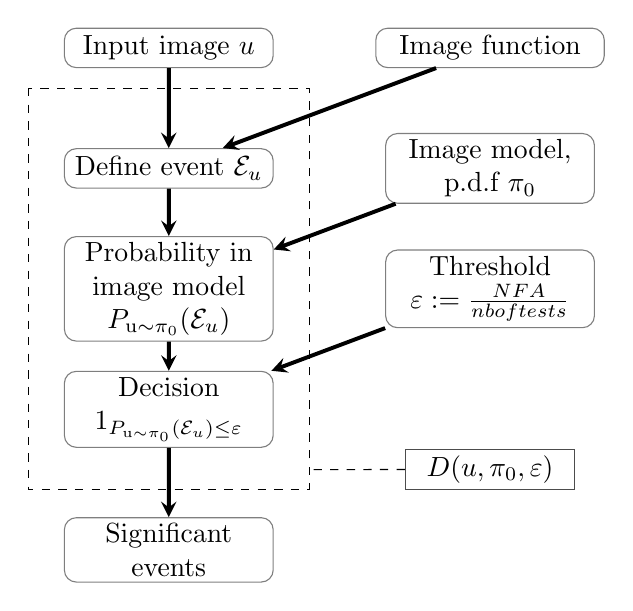
\begin{tikzpicture}[scale=1.02]
  \node[draw, minimum width = 1cm, minimum height = 0.5cm, text width=2.5cm, align=center, inner sep=0.5ex, rounded corners=1ex, fill=white, opacity=.5, text opacity = 1] (node 1) at (0.5,7) {Input image $u$};
  \node[draw, minimum width = 1cm, minimum height = 0.5cm, text width=2.5cm, align=center, inner sep=0.5ex, rounded corners=1ex, fill=white, opacity=.5, text opacity = 1] (node 2) at (0.5,5.5) {Define event $\mathcal{E}_u$};
  \node[draw, minimum width = 1cm, minimum height = 0.5cm, text width=2.5cm, align=center, inner sep=0.5ex, rounded corners=1ex, fill=white, opacity=.5, text opacity = 1] (node 3) at (0.5,4) {Probability in image model $P_{\bm{\mathrm{u}} \sim \pi_0}(\mathcal{E}_u)$};
  \node[draw, minimum width = 1cm, minimum height = 0.5cm, text width=2.5cm, align=center, inner sep=0.5ex, rounded corners=1ex, fill=white, opacity=.5, text opacity = 1] (node 4) at (0.5,2.5) {Decision $\mathbb{1}_{P_{\bm{\mathrm{u}} \sim \pi_0}(\mathcal{E}_u) \le \varepsilon}$};
  \node[draw, minimum width = 1cm, minimum height = 0.5cm, text width=2.5cm, align=center, inner sep=0.5ex, rounded corners=1ex, fill=white, opacity=.5, text opacity = 1] (node 5) at (0.5,0.75) {Significant events};
  

  \node[draw, minimum width = 1cm, minimum height = 0.5cm, text width=2.75cm, align=center, inner sep=0.5ex, rounded corners=1ex, fill=white, opacity=.5, text opacity = 1] (node 6) at (4.5,7) {Image function};
  \node[draw, minimum width = 1cm, minimum height = 0.5cm, text width=2.5cm, align=center, inner sep=0.5ex, rounded corners=1ex, fill=white, opacity=.5, text opacity = 1] (node 7) at (4.5,5.5) {Image model, p.d.f $\pi_0$};
  \node[draw, minimum width = 1cm, minimum height = 0.5cm, text width=2.5cm, align=center, inner sep=0.5ex, rounded corners=1ex, fill=white, opacity=.5, text opacity = 1] (node 8) at (4.5,4) {Threshold ${\varepsilon:= \frac{\operatorname{NFA}}{\text{nb of tests}}}$};

  
  \node[draw, minimum width = 1cm, minimum height = 0.5cm, text width=2cm, align=center, inner sep=0.5ex, fill=white, opacity=.7, text opacity = 1] (node 9) at (4.5,1.75) {$D(u,\pi_0,\varepsilon)$};  
  
  \draw [->, line width=.5mm,>=stealth, black] (node 1) -- (node 2);
  \draw [->, line width=.5mm,>=stealth, black] (node 2) -- (node 3);
  \draw [->, line width=.5mm,>=stealth, black] (node 3) -- (node 4);
  \draw [->, line width=.5mm,>=stealth, black] (node 4) -- (node 5);
  \draw [->, line width=.5mm,>=stealth, black] (node 6) -- (node 2);
  \draw [->, line width=.5mm,>=stealth, black] (node 7) -- (node 3);
  \draw [->, line width=.5mm,>=stealth, black] (node 8) -- (node 4);

  \draw[dashed] (-1.25,6.5) rectangle (2.25,1.5);

  \draw [dashed, black] (node 9) -- (2.25,1.75);
  
  % % general arrows
  % \node[draw, double arrow, shade, shading=axis, left color=white,right color=black,
  % minimum height=155mm, minimum width=5mm,
  % single arrow head extend=2mm,
  % anchor=west, rotate=0] at (-0.5,0) {};
  % \node[draw, single arrow, shade , shading=axis, bottom color=white,top color=black,
  % minimum height=145mm, minimum width=5mm,
  % single arrow head extend=2mm,
  % anchor=west, rotate=-90] at (-2,15) {};

  % % draw nodes
  % \node[draw, minimum width=4cm] (node 1) at (1,13) {sub-invariant measure};
  % \node[draw, minimum width=4cm] (node 2) at (1,10.75) {$\forall x \in X, \forall A \in \mathcal{B}, Q(x,A)=1$};              
  % \node[draw, minimum width=4cm] (node 3) at (1,9.25) {invariant measure};
  % \node[draw, minimum width=4cm] (node 4) at (1,7.75) {$\forall A \in \mathcal{B}, \underset{x \in X}{\sup}E_x(\tau_A) < +\infty$};
  % \node[draw, minimum width=4cm] (node 5) at (1,6.25) {invariant probability};
  % \node[draw, minimum width=4cm] (node 6) at (1,5) {strong aperiodicity};
  % \node[draw, minimum width=4cm] (node 7) at (1,3) {geometric recurrence};              
  % \node[draw, minimum width=3.2cm] (node 8) at (6.5,15) {Feller type condition};
  % \node[draw, minimum width=3.2cm] (node 9) at (6.5,13) {$\varphi$-irreducibility};    
  % \node[draw, minimum width=3.2cm] (node10) at (7,10) {Harris recurrence};
  % \node[draw, minimum width=3.2cm] (node11) at (7,7) {Harris positive recurrence};
  % \node[draw, minimum width=3.2cm] (node12) at (7,5) {Harris ergodicity};
  % \node[draw, minimum width=3.2cm] (node13) at (7,3) {geometric ergodicity};              
  % \node[draw, minimum width=3.2cm] (node14) at (12.5,15) {all compact sets are petite};              
  % \node[draw, minimum width=3.2cm] (node15) at (12.5,13) {$T$-chain};              
  % \node[draw, minimum width=3.2cm] (node16) at (12,10) {non-evanescence};
  % \node[draw, minimum width=3.2cm] (node17) at (12,7) {bounded probability};              
  % \node[draw] (node18) at (15,10) {DD1};
  % \node[draw] (node19) at (15,7) {DD2};
  % \node[draw] (node20) at (15,3) {DD3};
  % \node[draw] (node21) at (15,1) {DD4};

  % % intermediate node
  % \node[fill=black, minimum size=1pt] (node22) at (9.5,13) {};

  % % draw boxes
  % \draw[dashed] (4.5,10.5) rectangle (14,6.5);
  % \draw[dashed] (4.5,5.5) rectangle (14,2.5);

  % % draw logical arrows
  % \draw [->, line width=1mm,>=stealth, black] (node14) -- node[shape=circle, draw, inner sep=1pt, line width=1pt, right=3pt, fill=white] {4} (node15);
  % \draw [<->, line width=1mm, >=stealth, black] (node10) -- node[shape=circle, draw, inner sep=1pt, line width=1pt, below=3pt, fill=white] {5}(node16);
  % \draw [<->, line width=1mm, >=stealth, black] (node11) -- node[shape=circle, draw, inner sep=1pt, line width=1pt, below=3pt, fill=white] {5} (node17);    
  % \draw [->, line width=1mm, >=stealth, black] (node18) -- node[shape=circle, draw, inner sep=1pt, line width=1pt, below=3pt, fill=white] {6}(node16);
  % \draw [->, line width=1mm, >=stealth, black] (node19) -- node[shape=circle, draw, inner sep=1pt, line width=1pt, below=3pt, fill=white, fill = white] {7}(node17);
  % \draw [->, line width=1mm, >=stealth, black] (node20) -- node[shape=circle, draw, inner sep=1pt, line width=1pt, below=3pt, fill=white] {10}(node13);
  % \draw [->, line width=1mm, >=stealth, black] (node 7) -- node[shape=circle, draw, inner sep=1pt, line width=1pt, below=3pt, fill=white] {9} (node13);    
  % \draw [->, line width=1mm, >=stealth, black] (node21) -- (node20);
  % \draw [->, line width=1mm, >=stealth, black] (node11) -- node[shape=circle, draw, inner sep=1pt, line width=1pt, right=3pt, fill=white] {8} (node12);
  % \draw [->, line width=1mm, >=stealth, black] (node11) |- (node 5);
  % \draw [->, line width=1mm, >=stealth, black] (node 4) -| (node11);
  % \draw [->, line width=1mm, >=stealth, black] (node 2) -| (node10);
  % \draw [->, line width=1mm, >=stealth, black] (node10) |- node[shape=circle, draw, inner sep=1pt, line width=1pt, below=3pt, fill=white] {2} (node 3);
  % \draw [->, line width=1mm, >=stealth, black] (node 8) -- node[shape=circle, draw, inner sep=1pt, line width=1pt, below=3pt, fill=white] {3} (node14);
  % \draw [->, line width=1mm, >=stealth, black] (node 9) -- node[shape=circle, draw, inner sep=1pt, line width=1pt, below=3pt, fill=white] {1}(node 1);

  % % other nodes
  % \draw [-, black] (node 9) -- (node22);
  % \draw [-, black] (node15) -- (node22);
  % \draw [-, black] (node22) -- (9.5,10.5);
  % \draw [-, black] (node 6) -- (4.5,5);

  % % axis
  % \node at (1,-0.5) {\textbf{probability}};
  % \node at (13.5,-0.5) {\textbf{topology}};
  % \node[rotate = 90] at (-2.5,2) {\textbf{ergodicity}};
  % \node[rotate = 90] at (-2.5,14) {\textbf{stability}};    

\end{tikzpicture}
\end{flushleft}

%%% Local Variables:
%%% mode: latex
%%% TeX-master: "../../../../latex/report_thesis"
%%% End:
%%% Local Variables:
%%% mode: latex
%%% TeX-master: "main"
%%% End:
